\documentclass{wissdoc}
% Autor: Florian Weber 2013-2014, weberflorian <at> me.de
% Vorlagenautor: Roland Bless 1996-2009, bless <at> kit.edu
% ----------------------------------------------------------------
% Diplomarbeit - Hauptdokument‚
% ----------------------------------------------------------------
%%
%% $Id: thesis.tex 65 2012-05-10 10:32:11Z bless $
%%
% wissdoc Optionen: draft, relaxed, pdf --> siehe wissdoc.cls
% ------------------------------------------------------------------
% Weitere packages: (Dokumentation dazu durch "latex <package>.dtx")
\usepackage[numbers,sort&compress]{natbib}
\usepackage{float}
\restylefloat{table} %!damit tabellen dort auftauchen, wo sie beschrieben werden([H] benutzen!)
\usepackage[official]{eurosym} % für Eurosymbol
\usepackage{listings} %für Quellcode
\lstset{
  literate={Ö}{{\"O}}1
{Ä}{{\"A}}1
{Ü}{{\"U}}1
{ß}{{\ss}}2
{ü}{{\"u}}1
{ä}{{\"a}}1
{ö}{{\"o}}1
}
% \usepackage{varioref}
% \usepackage{verbatim}
% \usepackage{float}    %z.B. \floatstyle{ruled}\restylefloat{figure}
% \usepackage{subfigure}
% \usepackage{fancybox} % für schattierte,ovale Boxen etc.
% \usepackage{tabularx} % automatische Spaltenbreite
% \usepackage{supertab} % mehrseitige Tabellen
% \usepackage[svnon,svnfoot]{svnver} % SVN Versionsinformation 
%% ---------------- end of usepackages -------------

%\svnversion{$Id: thesis.tex 65 2012-05-10 10:32:11Z bless $} % In case that you want to include version information in the footer

%% Informationen für die PDF-Datei
\hypersetup{
 pdfauthor={Florian Weber},
 pdftitle={Kostencontrolling bei T-Systems am Kundenbeispiel}
 pdfsubject={Expose zur Bachelorarbeit},
 pdfkeywords={Not set}
}

% Macros, nicht unbedingt notwendig
%%%%%%%%%%%%%%%%%%%%%%%%%%%%%%%%%%%%%%%%%%%%%%%%%%%%%%%%%%
% macros.tex -- einige mehr oder weniger nuetzliche Makros
% Autor: Roland Bless 1998
%%%%%%%%%%%%%%%%%%%%%%%%%%%%%%%%%%%%%%%%%%%%%%%%%%%%%%%%%%
% $Id: macros.tex 33 2007-01-23 09:00:59Z bless $
%%%%%%%%%%%%%%%%%%%%%%%%%%%%%%%%%%%%%%%%%%%%%%%%%%%%%%%%%%


%%%%%%%%%%%%%%%%%%%%%%%
% Kommentare 
%%%%%%%%%%%%%%%%%%%%%%%
\ifnotdraftelse{
\newcommand{\Kommentar}[1]{}
}{\newcommand{\Kommentar}[1]{{\em #1}}}
% Alles innerhalb von \Hide{} oder \ignore{} 
% wird von LaTeX komplett ignoriert (wie ein Kommentar)
\newcommand{\Hide}[1]{}
\let\ignore\Hide

%%%%%%%%%%%%%%%%%%%%%%%%%
% Leere Seite ohne Seitennummer, wird aber gezaehlt
%%%%%%%%%%%%%%%%%%%%%%%%%

\newcommand{\leereseite}{% Leerseite ohne Seitennummer, nächste Seite rechts (wenn 2-seitig)
 \clearpage{\pagestyle{empty}\cleardoublepage}
}
%%%%%%%%%%%%%%%%%%%%%%%%%%
% Flattersatz rechts und Silbentrennung, Leerraum nach rechts maximal 1cm
%%%%%%%%%%%%%%%%%%%%%%%%%%
\makeatletter
\newcommand{\myraggedright}{%
 \let\\\@centercr\@rightskip 0pt plus 1cm
 \rightskip\@rightskip
  \leftskip\z@skip
  \parindent\z@
  \spaceskip=.3333em
  \xspaceskip=.5em}
\makeatother

\makeatletter
\newcommand{\mynewline}{%
 \@centercr\@rightskip 0pt plus 1cm
}
\makeatother


%%%%%%%%%%%%%%%%%%%%%%%%%%
% Für Index
%%%%%%%%%%%%%%%%%%%%%%%%%%
\makeatletter
\def\mydotfill{\leavevmode\xleaders\hb@xt@ .44em{\hss.\hss}\hfill\kern\z@}
\makeatother
\def\bold#1{{\bfseries #1}}
\newbox\dbox \setbox\dbox=\hbox to .4em{\hss.\hss} % dot box for leaders
\newskip\rrskipb \rrskipb=.5em plus3em % ragged right space before break
\newskip\rrskipa \rrskipa=-.17em plus -3em minus.11em % ditto, after
\newskip\rlskipa \rlskipa=0pt plus3em % ragged left space after break
\newskip\rlskipb \rlskipb=.33em plus-3em minus.11em % ragged left before break
\newskip\lskip \lskip=3.3\wd\dbox plus1fil minus.3\wd\dbox % for leaders
\newskip \lskipa \lskipa=-2.67em plus -3em minus.11em %after leaders
\mathchardef\rlpen=1000 \mathchardef\leadpen=600
\def\rrspace{\nobreak\hskip\rrskipb\penalty0\hskip\rrskipa}
\def\rlspace{\penalty\rlpen\hskip\rlskipb\vadjust{}\nobreak\hskip\rlskipa}
\let\indexbreak\rlspace
\def\raggedurl{\penalty10000 \hskip.5em plus15em \penalty0 \hskip-.17em plus-15em minus.11em}
\def\raggeditems{\nobreak\hskip\rrskipb \penalty\leadpen \hskip\rrskipa %
\vadjust{}\nobreak\leaders\copy\dbox\hskip\lskip %
\kern3em \penalty\leadpen \hskip\lskipa %
\vadjust{}\nobreak\hskip\rlskipa}
\renewcommand*\see[2]{\rlspace\emph{\seename}~#1} % from makeidx.sty

%%%%%%%%%%%%%%%%%%%%%%%%%%
% Neue Seite rechts, leere linke Seite ohne Headings
%%%%%%%%%%%%%%%%%%%%%%%%%%
\newcommand{\xcleardoublepage}
{{\pagestyle{empty}\cleardoublepage}}

%%%%%%%%%%%%%%%%%%%%%%%%%%
% Tabellenspaltentypen (benoetigt colortbl)
%%%%%%%%%%%%%%%%%%%%%%%%%%
\newcommand{\PBS}[1]{\let\temp=\\#1\let\\=\temp}
\newcolumntype{y}{>{\PBS{\raggedright\hspace{0pt}}}p{1.35cm}}
\newcolumntype{z}{>{\PBS{\raggedright\hspace{0pt}}}p{2.5cm}}
\newcolumntype{q}{>{\PBS{\raggedright\hspace{0pt}}}p{6.5cm}}
\newcolumntype{g}{>{\columncolor[gray]{0.8}}c} % Grau
\newcolumntype{G}{>{\columncolor[gray]{0.9}}c} % helleres Grau

%%%%%%%%%%%%%%%%%%%%%%%%%%
% Anführungszeichen oben und unten
%%%%%%%%%%%%%%%%%%%%%%%%%%
\newcommand{\anf}[1]{"`{#1}"'}

%%%%%%%%%%%%%%%%%%%%%%%%%%
% Tiefstellen von Text
%%%%%%%%%%%%%%%%%%%%%%%%%%
% S\tl{0} setzt die 0 unter das S (ohne Mathemodus!)
% zum Hochstellen gibt es uebrigens \textsuperscript
\makeatletter
\DeclareRobustCommand*\textlowerscript[1]{%
  \@textlowerscript{\selectfont#1}}
\def\@textlowerscript#1{%
  {\m@th\ensuremath{_{\mbox{\fontsize\sf@size\z@#1}}}}}
\let\tl\textlowerscript
\let\ts\textsuperscript
\makeatother

%%%%%%%%%%%%%%%%%%%%%%%%%%
% Gauß-Klammern
%%%%%%%%%%%%%%%%%%%%%%%%%%
\newcommand{\ceil}[1]{\lceil{#1}\rceil}
\newcommand{\floor}[1]{\lfloor{#1}\rfloor}

%%%%%%%%%%%%%%%%%%%%%%%%%%
% Average Operator (analog zu min, max)
%%%%%%%%%%%%%%%%%%%%%%%%%%
\def\avg{\mathop{\mathgroup\symoperators avg}}

%%%%%%%%%%%%%%%%%%%%%%%%%%
% Wortabkürzungen
%%%%%%%%%%%%%%%%%%%%%%%%%%
\def\zB{z.\,B.\ }
\def\dh{d.\,h.\ }
\def\ua{u.\,a.\ }
\def\su{s.\,u.\ }
\newcommand{\bzw}{bzw.\ }

%%%%%%%%%%%%%%%%%%%%%%%%%%%%%%%%%%%
% Einbinden von Graphiken
%%%%%%%%%%%%%%%%%%%%%%%%%%%%%%%%%%%
% global scaling factor
\def\gsf{0.9}
%% Graphik, 
%% 3 Argumente: Datei, Label, Unterschrift
\newcommand{\Abbildung}[3]{%
\begin{figure}[tbh] %
\centerline{\scalebox{\gsf}{\includegraphics*{#1}}} %
\caption{#3} %
\label{#2} %
\end{figure} %
}
\let\Abb\Abbildung
%% Abbps
%% Graphik, skaliert, Angabe der Position
%% 5 Argumente: Position, Breite (0 bis 1.0), Datei, Label, Unterschrift
\newcommand{\Abbildungps}[5]{%
\begin{figure}[#1]%
\begin{center}
\scalebox{\gsf}{\includegraphics*[width=#2\textwidth]{#3}}%
\caption{#5}%
\label{#4}%
\end{center}
\end{figure}%
}
\let\Abbps\Abbildungps
%% Graphik, Angabe der Position, frei wählbares Argument für includegraphics
%% 5 Argumente: Position, Optionen, Datei, Label, Unterschrift
\newcommand{\Abbildungpf}[5]{%
\begin{figure}[#1]%
\begin{center}
\scalebox{\gsf}{\includegraphics*[#2]{#3}}%
\caption{#5}%
\label{#4}%
\end{center}
\end{figure}%
}
\let\Abbpf\Abbildungpf

%%
% Anmerkung: \resizebox{x}{y}{box} skaliert die box auf Breite x und Höhe y,
%            ist x oder y ein !, dann wird das usprüngliche 
%            Seitenverhältnis beibehalten.
%            \rescalebox funktioniert ähnlich, nur das dort ein Faktor
%            statt einer Dimension angegeben wird.
%%
% \Abbps{Position}{Breite in Bruchteilen der Textbreite}{Dateiname}{Label}{Bildunterschrift}
%

\newcommand{\refAbb}[1]{%
s.~Abbildung \ref{#1}}

%%%%%%%%%%%%%%%%%%%%
%% end of macros.tex
%%%%%%%%%%%%%%%%%%%%

% Print URLs not in Typewriter Font
\def\UrlFont{\rm}

%\newcommand{\blankpage}{% Leerseite ohne Seitennummer, nächste Seite rechts
% \clearpage{\pagestyle{empty}\cleardoublepage}
%}

%% Einstellungen für das gesamte Dokument

% Trennhilfen
% Wichtig! 
% Im ngerman-paket sind zusätzlich folgende Trennhinweise enthalten:
% "- = zusätzliche Trennstelle
% "| = Vermeidung von Ligaturen und mögliche Trennung (bsp: Schaf"|fell)
% "~ = Bindestrich an dem keine Trennung erlaubt ist (bsp: bergauf und "~ab)
% "= = Bindestrich bei dem Worte vor und dahinter getrennt werden dürfen
% "" = Trennstelle ohne Erzeugung eines Trennstrichs (bsp: und/""oder)

% Trennhinweise fuer Woerter hier beschreiben
\hyphenation{
% Pro-to-koll-in-stan-zen
Management  
% Netz-werk-ele-men-ten
% Netz-werk Netz-werk-re-ser-vie-rung
% Netz-werk-adap-ter Fein-ju-stier-ung
% Da-ten-strom-spe-zi-fi-ka-tion Pa-ket-rumpf
% Kon-troll-in-stanz
}

% Index-Datei öffnen
\ifnotdraft{\makeindex}
%%%%%%%%%%%%%% includeonly %%%%%%%%%%%%%%%%%%%
% Es werden nur die Teile eingebunden, die hier 
% aufgefuehrt sind!
\includeonly{%
titelseite,%
Problemstellung,% Motivation, Zielsetzung, Gliederung
Theoretischen_Bezug,% Grundlagen 
Fragestellung,% Grundlagen 
Methodik,% Grundlagen
Gliederungsentwurf,% Grundlagen
Zeitplan,% Grundlagen
}
%%%%%%%%%%%%%%%%%%%%%%%%%%%%%%%%%%%%%%%%%%%%%%
\begin{document}

\frontmatter
\pagenumbering{roman}
\ifnotdraft{
 %% Titelseite
%% Vorlage $Id: titelseite.tex 61 2012-05-03 13:58:03Z bless $

\def\usesf{}
\let\usesf\sffamily % diese Zeile auskommentieren für normalen TeX Font

\newsavebox{\Erstgutachter}
\savebox{\Erstgutachter}{\usesf Prof. Dr. rer. pol.~Ingolf \textsc{Weise}}
\newsavebox{\Zweitgutachter}
\savebox{\Zweitgutachter}{\usesf Dipl.-Wi.-Math.~Dirk \textsc{Espinoza}}
\newsavebox{\Studiengang}
\savebox{\Studiengang}{\usesf Wirtschaftsinformatik (B.Sc.)}

\begin{titlepage}
\setlength{\unitlength}{1pt}
\begin{picture}(0,0)(85,770)

\includegraphics[width=\paperwidth]{logos/HFTL_Deckblatt}
\end{picture}

\thispagestyle{empty}

%\begin{titlepage}
%%\let\footnotesize\small \let\footnoterule\relax
\begin{center}
\hbox{}
\vfill
{\usesf
{\LARGE\bfseries 
              Exposé zur Bachelorarbeit \par}
\vskip 1.8cm
{\Large\bfseries
Kostencontrolling bei T-Systems \\
am Kundenbeispiel \\}
von\\[2mm]
\vskip 1cm

{\large\bfseries Florian Weber\\}
Moosburger Str. 19a\\
85276 Pfaffenhofen\\
florian.weber@hft-leipzig.de\\
\vskip 1.2cm
an der Hochschule für Telekommunikation Leipzig\\
der Fakultät für Informatik\
%Universität Karlsruhe (TH)\\[2ex]
\vskip 3cm
\begin{tabular}{p{5.5cm}l}
Betreuender Professor: & \usebox{\Erstgutachter} \\
Zweitprüfer: & \usebox{\Zweitgutachter}\\
Studiengang: & \usebox{\Studiengang}\\
\vskip 3cm
Version: 1.0\\
Stand: 27.07.2014
\end{tabular}
\vskip 5cm
}
\end{center}
\vfill
\end{titlepage}
%% Titelseite Ende


%%% Local Variables: 
%%% mode: latex
%%% TeX-master: "thesis"
%%% End: 

}
%% *************** Hier geht's ab ****************
%% ++++++++++++++++++++++++++++++++++++++++++
%% Verzeichnisse
%% ++++++++++++++++++++++++++++++++++++++++++
\ifnotdraft{
{\parskip 0pt\tableofcontents} % toc bitte einzeilig
%\blankpage
%\listoffigures
%\blankpage
%\listoftables
%\blankpage
}


%% ++++++++++++++++++++++++++++++++++++++++++
%% Hauptteil
%% ++++++++++++++++++++++++++++++++++++++++++
\graphicspath{{Bilder/}}

\mainmatter
\pagenumbering{arabic}
%% Problemstellung.tex
%% $Id: Problemstellung.tex 61 2012-05-03 13:58:03Z bless $
%%


\chapter{Problemstellung und eigenes Erkenntnisinteresse}
\label{ch:Problemstellung}

Aufgrund von aktuellen Gegebenheiten bei der Deutschen Telekom AG mit Kostensenkungen und Umstrukturierung oder dem Stellenabbau bei T –Systems \cite{web:Handelsblatt}, stellt sich die Frage nach der Anwendung des Controllings sowie den Unterschied zwischen Theorie, Konzeption und Praxis.
\\
\\
Durch den Einsatz des Autors als dualer Student bei T-Systems im Service Delivery Management wurde dessen Arbeitsumfeld erlebt.
Die Aufgabe im Service Delivery Management ist nach ITIL unter anderem die Begleitung des IT Service Lebenszyklus \cite{web:LiveCylce} in all deren Phasen.
Von Service Strategie, über Service Design, Service Transition, Service Operation bis hin zur Kontinuierlichen Service Verbesserung.
\\
\\
Hier tritt das erste Problem auf, denn das Ziel vieler Unternehmen ist es Kunden langfristig an sich zu binden um nachhaltige Wettbewerbsvorteile zu schaffen. 
\\
Um dem internationalen Druck der Konkurrenz im IT Sourcing standzuhalten, ist neben einem Umfangreichen Portfolio, durchgängiger Verfügbarkeit und umfassenden "Know How", eine Finanzielle Strategie für den gesamten Lebenszyklus zu entwickeln.
Dabei ist es fundamental die erarbeitete Strategie im Anschluss zu steuern.
Es gilt ein Zielsystem für die Budgetierung zu planen und dabei Planungsschritte und Unterlagen zu erstellen.
Des Weiteren ein Informationssystem für das Management zu organisieren, um das Fundament zur Beurteilung der Wirtschaftlichkeit und Geschäftsentwicklung an Kennzahlen der Betriebswirtschaftslehre zu legen.
Im Nachhinein wird die Entwicklung an aufgestellten Kennzahlen überprüft und mit festgelegten Maßnahmen gesteuert.
Hierbei werden unter anderem Soll-Ist-Vergleiche durchgeführt und die Ursachen für Abweichungen vom Controller ermittelt und analysiert um Prognosen abgeben zu können.
Die definierten Maßnahmen werden vom Controller koordiniert und in den einzelnen Teilbereichen angepasst.
\\
\\
Um mit internen sowie externen Kosten für die Erbringung des Services kalkulieren einzuhalten und die Notwendigkeit positive Geschäftszahlen erreichen zu können, werden die dargestellten Controlling \cite{web:Controlling} Aufgaben ebenfalls innerhalb des Service Delivery Managements übernommen.
\\
\\
Die dargestellten Informationen und Probleme veranschaulichen Bedarf das Kostencontrolling von T-Systems näher zu untersuchen.




%%% Local Variables: 
%%% mode: latex
%%% TeX-master: "thesis"
%%% End: 
  				% Problemstellung
%% Theoretischen_Bezug.tex
%% $Id: Theoretischen_Bezug.tex 61 2012-05-03 13:58:03Z bless $
%%

\chapter{Theoretischen Bezug und bisheriger Forschungsstand }
\label{ch:Theoretischen_Bezug}


Zum derzeitigen Zeitpunkt gibt es unterschiedliche Ansätze der Forschung im Controlling, speziell in der Konzeption. In den letzten 20 Jahren hat sich zudem die Ausrichtung weg von einer rein wirtschaftlichen Teildisziplin bis hin zur eigenständigen Controlling Funktion entwickelt.
\\
Wie bereits in Punkt eins erwähnt stellt sich die Frage nach dem Unterschied im Controlling zwischen Theorie, Konzeption und Praxis. Wie in Abbildung \ref{fig:Controllingkonzeption} zu sehen ist, gibt es nach Scherm und Pietsch gibt es eine große Anzahl an Konzeptionen die zwischen klassischen und neuen Konzeptionen des Controllings unterschieden werden.

\begin{figure}[H]
 \centering
 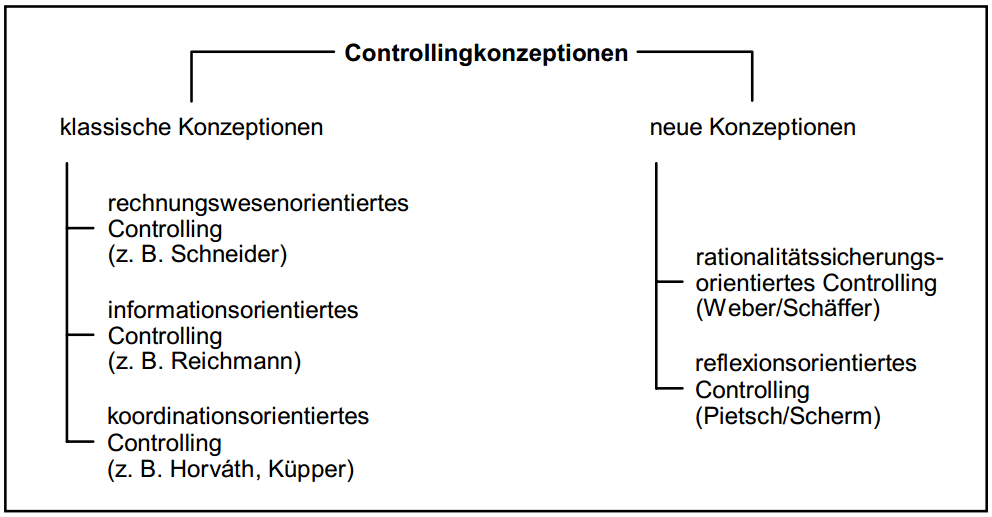
\includegraphics[scale=0.45]{images/Controllingkonzeption.png}
 \caption{Controllingkonzeptionen \cite{fig:Controllingkonzeption}}
 \label{fig:Controllingkonzeption}
\end{figure}

Während sich die klassischen Konzeptionen auf Rechnungswesen orientiertes, informationsorientiertes und koordinationsorientiertes Controlling die klassischen Konzeptionen wiederspiegeln, handelt es bei den neuen Konzeptionen um jene, die sich mit Entscheidungen und Sicherstellung der Führungsrationalität befasst.
\\
Diese Konzeptionen können mit den Kundenorientierten Controlling Ansätzen innerhalb der T-Systems verglichen werden.


%%% Local Variables: 
%%% mode: latex
%%% TeX-master: "thesis"
%%% End: 
     		% Theorie ITIL
%% Fragestellung.tex
%% $Id: Fragestellung.tex 61 2012-05-03 13:58:03Z bless $
%%

\chapter{Fragestellung oder Hypothese}
\label{ch:Fragestellung}

Dieses Kapitel beschäftigt sich mit den einzelnen Fragestellungen die sich bis hin zur Bachelorthesis hin entwickelt. 
Aus den in Punkt ein und Punkt zwei genannten Theoretischen Grundlagen sowie den unterschiedlichen Einsatzbereichen des Controllings ergeben sich folgende Fragstellungen:
\begin{quote}
1. Fragestellung: 
Welche Philosophie beinhaltet das Controlling?
\end{quote}

Dieser Abschnitt soll die Problemstellung verdeutlichen und die Controlling Theorie, Controlling Konzeptionen und Philosophie des Kostencontrolling sowie der Hintergrund verdeutlichen.
Aufgrund der Beantwortung dieser Frage und die somit verbundene Verdeutlichung des Themas, ergibt sich folgende Fortsetzung:
\begin{quote}
2. Fragestellung: 
Welche Treiber gibt es in der deutschen Wirtschaft für Kostencontrolling?
\end{quote}

Hier werden die treibenden Unternehmen und Anreize für Kostencontrolling der deutschen Wirtschaft wiedergespiegelt. Darüber hinaus sollen mögliche Tools und Software für Controlling erläutert werden sowie die Controlling Instrumente und Anwendungsbereiche in Unternehmen aufgezeigt werden.
Nach diesen Erläuterungen soll auf den Spezialfall Bezug genommen werden, wodurch so folgende Fragestellung ergibt
\begin{quote}
3. Fragestellung: 
Wie ist das Controlling bei T-Systems aufgebaut?
\end{quote}

Diese Untersuchung gibt Aufschluss über das Profil der T-Systems und deren Anforderungen an das Kostencontrolling. Des Weiteren soll dieser Prozess wiedergespiegelt sowie dessen Umsetzung mit Hilfe von Angewandten Tools beschrieben werden.
\begin{quote}
4. Fragestellung: 
Wie gestaltet sich die Anwendung am Kundenbeispiel?
\end{quote}

Anschließend wird die theoretische Auslegung des Kostencontrollings bei T-Systems anhand eines gezielten Kundenbeispiels beschrieben. Dies wird anhand einer empirischen Erhebung des IST-Zustandes mithilfe des Kundenbeispiels beschrieben. Dadurch ergibt sich die grundlegende Fragestellung der Arbeit:
\begin{quote}
5. Fragestellung: 
Welche Unterschiede ergeben sich zwischen Theorie und Praxis innerhalb der T-Systems?
\end{quote}

Hier werden die Unterschiede und Abweichung zwischen Theorie, Konzeption und Praxis erläutert und abschließend in Risiken und Benefiz sowie einem Ausblick auf weitere Fragestellungen beendet.


%%% Local Variables: 
%%% mode: latex
%%% TeX-master: "thesis"
%%% End: 
     			% Theorie ITIL
%% Methodik.tex
%% $Id: Methodik.tex 61 2012-05-03 13:58:03Z bless $
%%

\chapter{Methodik und Material}
\label{ch:Methodik}

Nachfolgend wird die Vorgehensweise zur Bearbeitung der Bachelorarbeit aufgeführt: 
\begin{center}
\begin{description}
\item[Inhaltsverzeichnis]~\par
\begin{itemize}
	\item Erklärung und Darstellung des Begriffes Controlling
	\begin{itemize}
		\item Darstellung der Theorie
		\item Darstellung der Instrumente
		\item Darstellung der Konzeptionen
		\item Erklärung der Philosophie von Kostencontrolling
	\end{itemize}
	\item Identifizierung von Antreibern in der deutschen Wirtschaft
	\begin{itemize}
		\item Identifizierung und Unternehmen
		\item Identifizierung und Beschreibung von möglichen Tools
		\item Identifizierung und Darstellung von Anwendungsbereichen
	\end{itemize}
	\item Erklärung und Darstellung der T-Systems
	\begin{itemize}
		\item Beschreibung des Unternehmensprofils
		\item Beschreibung der Anforderungen an das Kostencontrolling
		\item Beschreibung der Prozesssichtweise und geplanten Umsetzung
		\item Beschreibung der verwendeten Tools
	\end{itemize}
	\item Empirische Untersuchung
	\begin{itemize}
		\item Dokumentation und Beschreibung des angewandten Kundenprozesses
		\item Beschreibung der Umsetzung des Spezialfalls
		\item Beschreibung der Kennzahlen
	\end{itemize}
	\item Vergleiche
	\begin{itemize}
		\item Identifizierung und Beschreibung von Unterschieden zwischen Theorie und Praxis
		\item Identifizierung und Beschreibung von Unterschieden zwischen Theorie und Konzeption
	\end{itemize}
	\item Ermittlung der Zustimmung oder Ablehnung der formulierten Hypothesen
\end{itemize} 
\end{description}	
\end{center}

Im Mittelpunkt der Arbeit stehen die Erfassung der Theorie des Kostencontrollings sowie die empirische Analyse des Angewandten Prozesses bei T-Systems am Kundenbeispiel. Darüber hinaus liegt der Fokus auf dem Vergleich dieser ermittelten Informationen. 


%%% Local Variables: 
%%% mode: latex
%%% TeX-master: "thesis"
%%% End: 
     					% Theorie ITIL
%% Gliederungsentwurf.tex
%% $Id: Gliederungsentwurf.tex 61 2012-05-03 13:58:03Z bless $

\chapter{Gliederungsentwurf}
\label{ch:Gliederungsentwurf}
%% ==============================

Dieses Kapitel enthält die vorläufige Gliederung der Bachelorthesis und Zeigt den aktuellen IST-Zustand. Im Verlauf bis hin zur endgültigen Abgaben kann sich dieser Entwurf noch geringfügig andern. Der Gliederungsentwurf soll die aufgeführten Leitfaden in Punkt 3 beinhalten und diese beantworten.

\begin{center}
\begin{description}
\item[Inhaltsverzeichnis]~\par
\begin{enumerate}
	\item Einleitung
	\begin{enumerate}
         \item Problemstellung 
         \item Zielsetzung
         \item Aufbau und Vorgehensweise der Arbeit
    \end{enumerate}     
	\item Grundlagen zum Kostencontrolling
	\begin{enumerate}
         \item Controlling Theorie 
         \item Controlling Instrumente
         \item Controlling Konzeption
         \item Philosophie / Hintergrund Kostencontrolling
    \end{enumerate}     
	\item Antreiber innerhalb der deutschen Wirtschaft
	\begin{enumerate}
         \item Unternehmen
         \item Tools
         \item Anwendungsbereiche
    \end{enumerate}
	\item Hintergrund T-Systems
	\begin{enumerate}
         \item Unternehmensprofil
         \item Anforderungen an Kostencontrolling
         \item Prozesssichtweise der Umsetzung
         \item Angewandte Tools
    \end{enumerate}
	\item Kundenbeispiel
	\begin{enumerate}
         \item Anwendung
         \item Vorgehen
         \item Kennzahlen
    \end{enumerate}
	\item Vergleiche
	\begin{enumerate}
         \item Praxis – Theorie
         \item Praxis – Konzeption 
    \end{enumerate}
	\item Zusammenfassung
	\begin{enumerate}
         \item Risiken \& Benefiz
         \item Fazit
    \end{enumerate}
\end{enumerate} 
\end{description}	
\end{center}
  
%%% Local Variables: 
%%% mode: latex
%%% TeX-master: "thesis"
%%% End: 
  			% Theorie ITIL
%% Zeitplan.tex
%% $Id: Zeitplan.tex 61 2012-05-03 13:58:03Z bless $

\chapter{Zeit- und Arbeitsplan}
\label{ch:Zeitplan}
%% ==============================

 
Die folgende Abbildung enthält den Zeit- und Arbeitsplan.

\begin{figure}[H]
 \centering
 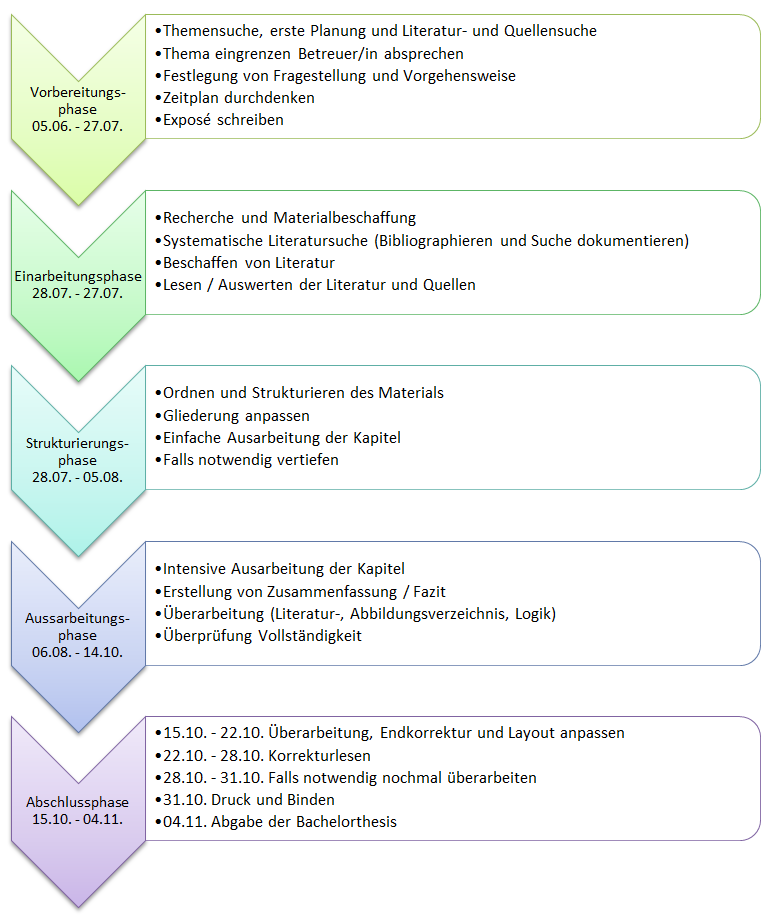
\includegraphics[scale=0.7]{images/Ablaufplan_BA.png}
 \caption{Ablaufplan der Vorgehensweise \cite{fig:Ablaufplan}}
 \label{fig:Ablaufplan}
\end{figure}

%%% Local Variables: 
%%% mode: latex
%%% TeX-master: "thesis"
%%% End: 
  					% Theorie ITIL


%% ++++++++++++++++++++++++++++++++++++++++++
%% Anhang
%% ++++++++++++++++++++++++++++++++++++++++++
\phantomsection
\appendix
%\include{
%\input{anhang_a}
%\input{anhang_b}}

%% ++++++++++++++++++++++++++++++++++++++++++
%% Literatur
%% ++++++++++++++++++++++++++++++++++++++++++
%  mit dem Befehl \nocite werden auch nicht 
%  zitierte Referenzen abgedruckt
\cleardoublepage
\phantomsection
\addcontentsline{toc}{chapter}{\bibname}
% $ bibtex thesis
%%
\nocite{*} % nur angeben, wenn auch nicht im Text zitierte Quellen 
           % erscheinen sollen
\bibliographystyle{ieeetr} % ausgeschriebene Vornamen der Autoren
%\bibliographystyle{gerplain} % abbrvnat unsrtnat
%\bibliographystyle{plainurl} % abbrvnat unsrtnat
% spezielle Zitierstile: Labels mit vier Buchstaben und Jahreszahl
%\bibliographystyle{ieeetr}  % mit abgekürzten Vornamen der Autoren
\bibliography{thesis}

\listoffigures
%\listoftables

%% ++++++++++++++++++++++++++++++++++++++++++
%% Index
%% ++++++++++++++++++++++++++++++++++++++++++
\ifnotdraft{
%\cleardoublepage
\phantomsection
\printindex            % Index, Stichwortverzeichnis
}
\end{document}
%% end of file
